%
%You can keep the 12pt font size, or go to 11pt or (default) 10pt
% Do NOT go any larger than 12pt font size for submission
%
%If you want to edit a printed copy, you may want to add draft mode
% (as in \documentclass[draft,conference,12pt]{IEEEtran})
% This adds space between the lines providing easier editing markup
%
%For more details see
% http://ras.papercept.net/conferences/support/files/IEEEtran_HOWTO.pdf
%
\documentclass[conference,11pt]{IEEEtran}
\usepackage{cite}
\usepackage{graphicx}
\usepackage{flushend}

% correct bad hyphenation here
\hyphenation{op-tical net-works semi-conduc-tor}

\begin{document}

%
% paper title
% Titles are generally capitalized except for words such as a, an, and, as,
% at, but, by, for, in, nor, of, on, or, the, to and up, which are usually
% not capitalized unless they are the first or last word of the title.
% Linebreaks \\ can be used within to get better formatting as desired.
% Do not put math or special symbols in the title.
\title{Programmatically Determining Optimal Scheduling Algorithms for Varying Process Sets}

\author{\IEEEauthorblockN{Rachael Engle, Anna Pankiewicz, and Albert Perlman}
\IEEEauthorblockA{Computer Science Department\\
Missouri University of Science and Technology\\
Rolla, MO 65409}}

% make the title area
\maketitle

\begin{abstract}
This work explores the advantages and disadvantages of using particular scheduling algorithms with different types of processes. The five specific algorithms analyzed were First In First Out, Round Robin, Shortest Job Next, Shortest Remaining Time, and Highest Response Ratio Next.
\end{abstract}

\section{Background}
Through the operating systems class this semester, each of these five scheduling algorithms were discussed. A high-level comparison was also provided in the lecture notes, highlighting differences in throughput, response time, overhead, effect on processes, and starvation.

While these given comparisons are useful, the purpose of our project was to implement these scheduling algorithms and observe the differences ourselves. As we are only simulating one processor and these are largely uniprocessor scheduling algorithms, some metrics are difficult to observe, such as throughput. However, by analyzing other metrics such as turnaround time, normalized turnaround time, and response time, we can gain insight into the more accessible performance metrics. Additionally, we can provide a quantifiable comparison of the average turnaround time for short, long, and mixed process sets using each specified algorithm.

\section{Introduction}
Our simulation centered around a system capable of handling incoming jobs, scheduling them, and allowing the user to select a scheduling function. A simulated job file is provided at the command line, and this file contains the process names, arrival times, and execution times. For simplicity's sake, the execution time of a process is provided, as it would be outside the scope of the project to analyze previous jobs and their characteristics to provide even remotely accurate time estimates.

This aforementioned simulated system is not alone in handling process arrivals and requests. Along with the "system", there is a master scheduler that runs the selected algorithm until all incoming processes have been completed. Every time cycle, this scheduler checks for jobs arriving at the current time, adds them to the appropriate queue of the running scheduling algorithm, and provides a snapshot of the system state at that time. When all jobs are finished, the scheduler concludes and produces a report of the algorithm's performance on that process set.

Every process represented in our system had certain information associated with it, along with the provided arrival and execution times. These included the actual start time of the process, cumulative time spent executing on the processor, total run time, and end time. Each scheduling algorithm function is configured to only run once per time cycle, and the master scheduler is responsible for ensuring that all processes are finished. Upon exiting the program, the system generates reports for each algorithm used during the simulation.

\section{Algorithms}

\subsection{First In First Out}
Arguably, the most simple scheduling algorithm is First In First Out (FIFO). As processes arrive, they are added to a queue. When the processor finishes executing a job, the longest-waiting process from this queue is selected to run. In our implementation, this is a simple task, as the order of the processes passed to a specific scheduling algorithm is in order of arrival time. This approach requires little overhead, but it may be unfair to short processes if many long processes arrive first.

There are some metrics that were outside the given scope of our project. We were unable to compare the performance of FIFO on processor-bound processes vs. I/O bound processes, and we were unable to simulate multiple processors running simultaneously as they would on a real system. However, as these are largely uniprocessor scheduling algorithms, that concern is not as prevalent.

\subsection{Round Robin}
Round Robin (RR) utilizes the act of preemption to schedule processes. Each process is given a length of time, the time quantum, to complete its job. If the process cannot complete during the time given, it is moved and added to the end of queue to continue executing later. This method of scheduling helps prevent starvation of any process since each process gets slices of time for executing.

However, there are some disadvantages to RR. In our implementation, there is no priority for important processes. When a process arrives, it is placed in the queue and has the same time quantum as any other process. With smaller time quantums, a significant amount of time is spent on switching processes and can extend the normalized turn around time of the processes.

Specifically in our system, the next process is run for the time quantum and checked for completion. If the process has completed, the scheduler checks if the runtime exactly equals the time quantum. If they don't match, the system time is decremented by one to reflect the process only running for one time slice, and the simulation continues. If the process has not completed, it's moved to the back of the process queue for further execution. This approach does require slight overhead in handling the switching on and off the processor, but implementation is fairly straightforward.

\subsection{Shortest Job Next}
A simple non preemptive approach to uniprocessor scheduling is Shortest Job Next. Like FIFO, an entire process executes fully, but the method for choosing the next process is different. After a process completes, the scheduler looks at the execution time of the waiting processes and chooses the shortest time. That shortest-execution process is then handed off to the processor to complete.

In our implementation, we made some necessary adjustments according to the scope of this project. For simplicity's sake, we provided a process's execution time immediately. In more realistic implementations of this algorithm, various methods are used to provide running time estimates, such as averaging the execution times of previously seen and fairly similar processes\cite{Silberschatz}. Each possible method requires extra overhead to record and calculate these necessary values.

Another consideration in SJN scheduling is the possibility of starvation. With our project, job files had a definite number of processes, and more couldn't be dynamically added. In uses of this algorithm on real processors, longer jobs may experience starvation if more short jobs keep arriving. With our system, this is not the case, as all provided jobs will eventually execute.

\subsection{Shortest Remaining Time}
While SJN may be favorable among non-preemptive approaches, it can be improved upon using preemption, and that is achieved in the Shortest Remaining Time algorithm. The process with the shortest execution time is still chosen to run, but things may change when a new process arrives. If the new process's running time is shorter than the currently running process's, the current process is preempted and the new one is given to the processor.

Additionally, every iteration the remaining time is calculated for each process. If an existing process has a shorter execution time remaining than the current one, it is preempted. Once a process is done running its portion, its progress time is incremented by the difference between the system time and process arrival time.

\subsection{Highest Response Ratio Next}
A nonpreemptive approach that can avoid the possible starvation of Shortest Job Next is that of Highest Response Ratio Next. The decision of what process to select is based on the below ratio: \\

\begin{math}
ratio = \frac{time spent waiting + expected service time}{expected service time}
\end{math}\\

This approach factors in both the time a process has already spent waiting and its execution time, providing a balance that successfully avoids starvation. Even if short processes keep arriving, a long process that has been waiting a significant amount of time will still have a higher response ratio than the new processes, and therefore be handed off to the processor.

In our implementation, the ratio for each process available is calculated using its execution time and a comparison of its arrival time to the current system time. The process with the highest ratio is selected to run, and it subsequently completes.

\section{Results}
Using the reports that our system generates, we tested each scheduler using 3 different sets of jobs - ten short jobs, ten long jobs, and 10 mixed (short and long) jobs. During our tests, we discovered that Shortest Remaining Time was the scheduler with the best turn around time for all three jobs. Specifically for the short and mixed job list, SRT significantly outweighed the others in time, almost halving the turn around time in half. With the long job list, SRT and Shortest Job Next ran very close, producing nearly the same turn around time.

\begin{figure}
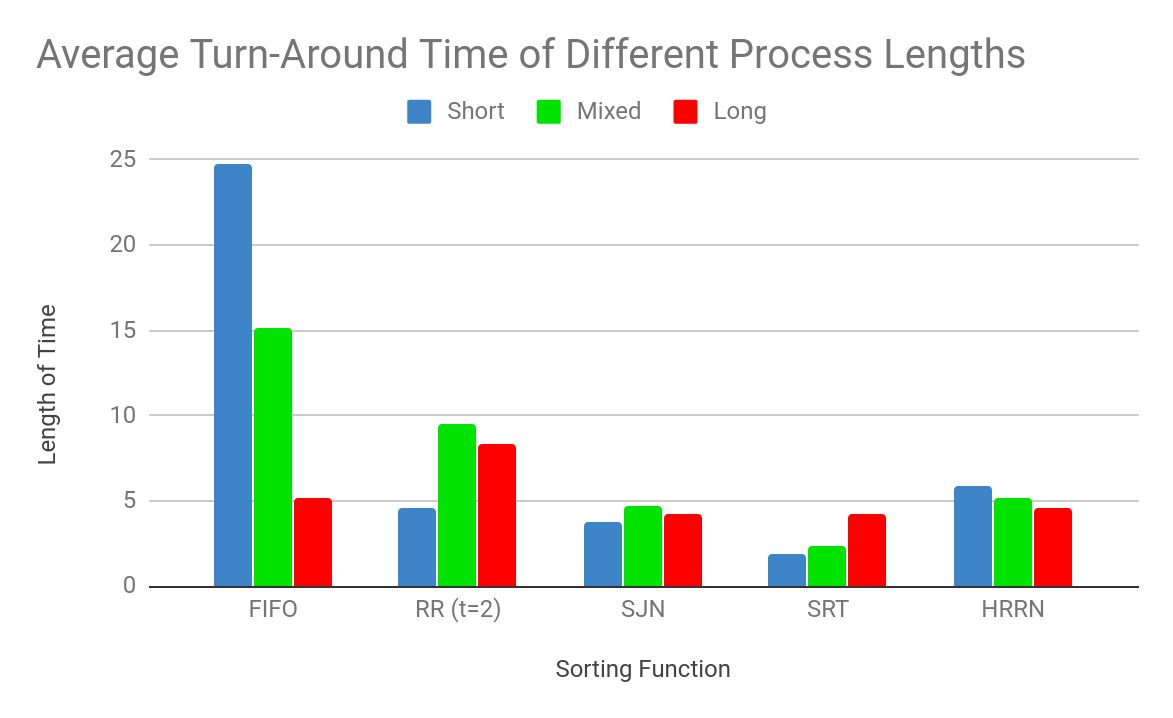
\includegraphics[width=\linewidth]{turnaround.png}
\caption{Average turnaround time for all schedulers.}
\label{fig:turnaround}
\end{figure}

Figure \ref{fig:turnaround} shows all turnaround time results. It's notable that Shortest Job Next, Shortest Remaining Time, and Highest Response Ratio Next individually have similar turnaround times for all process set lengths.

The worst scheduler to use for our jobs is First In First Out. It had the longest turn around time for the short and mixed job list. For the list of long jobs, Round Robin preformed the worst. With a time quantum of two, the turn around time was double all the other schedulers. However, with a time quantum of one hundred, the turn around time slightly increased from the other schedulers. The average turn around time only varied by .6 between the five different schedulers with a large time quantum. So, when the job list is full of very long processes, the scheduler used doesn't affect the total run time or turn around time in the end.

\bibliographystyle{ieeetr}
\begin{thebibliography}{3}
\bibitem{Silberschatz}
A. Silberschatz, P.B. Galvin, and G. Gagne,
\textit{Operating Systems Concepts}
Wiley, 7th ed., p. 161, 2005.
\end{thebibliography}

\end{document}
